\documentclass[10pt, conference]{IEEEtran}
\IEEEoverridecommandlockouts

\usepackage{times}
\usepackage{graphicx}
\usepackage{url}
\usepackage{color}
\usepackage{amsmath}
\usepackage{listings}

% \setlength{\textheight}{9.0in}
% \setlength{\textwidth}{6.50in}
% \setlength{\leftmargin}{1in}
% \setlength{\topmargin}{-0.5in}
% 
% \setlength\oddsidemargin{0in}
% \setlength\evensidemargin{0in}



% \title{Towards Self-Management in Distributed Application
% Management System \thanks{Supported by National Science
% Foundation of China (Grant No.~60603071) and National Basic
% Research Program of China (973, Grant No.~2007CB311100).}}

\title{SMON: Self-Managed Overlay Networks for Managing
Distributed Applications}

\author{\IEEEauthorblockN{Chongnan Gao$^\dag$, Hongliang
Yu$^\dag$, Guangyu Shiy$^\ddag$, Jian Chen$^\ddag$, Weimin Zheng$^\dag$}\\
\IEEEauthorblockA{$^\dag$Computer Science and Technology
Department, Tsinghua University, Beijing 10084, China\\
$^\ddag$Huawei Technologies Co., Ltd, Shenzhen, 518129, China\\
Email: gaochongnan@gmail.com, \{hlyu, zwm-dcs\}@tsinghua.edu.cn}\\

\thanks{Supported by National Natural
Science Foundation of China under Grant No.~60603071, the
Major State Basic Research Development Program of China (973
Program) under Grant No.~2007CB311100, National Key
Technology R\&D Program under grant No.~2006BAK15B10 and
Huawei Research Fund under contract No.~YBCB2009032.}}
\date{}

\newcommand{\note}[1]{{\textcolor{red}{{XXX: #1}}}}
\long\def\comment#1{}

\graphicspath{{figure/}}

\begin{document}

\maketitle
%\thispagestyle{empty}
%\pagestyle{empty}


\section*{Abstract}

Distributed application management system is important for
managing applications on distributed computing platforms. 
% The management system is designed in distributed approach
% and also need to be well monitored and maintained
% throughout its lifecycle. Currently, distributed
% management systems are monitored and maintained using
% centralized approach, which is not scalable and efficient.
One of the main caveat of using a distributed management
system is that the management system itself, as a
distributed application, need to be deployed and maintained
continually.  In this papar, we propose Self-Managed Overlay
Network (SMOM) and explore the challenges associated with
designing a management system with self-management
capability. SMON manages itself using epidemic approach at
runtime. SMON can automatically deploys itself to a set of
machines and recovers failed peers \emph{securely}. It can
also upgrade itself to new versions online. Through
mathematical analysis and evaluation on PlanetLab platform,
we show that SMON achieves good performance and scalability.

% vim:foldmethod=marker:textwidth=60

% vim:tw=60

\section{Introduction}
\label{sec:intro}

As industry is moving towards \textit{cloud computing}, many
players in the industry are building large and complex data
center applications on top of clusters of commodity PCs.
Ensuring the correctness and performance of the applications
are critical to providing sustained service to clients.
However, bugs have been challenging service developers and
maintainers continually.

However, the inherent complexity of the system hinders
people from understanding the system easily. The system are
usually built in a tiered fashion, with each tier providing
certain abstraction to the upper layer. Within a logical
tier, its function is implemented as a distributed system.
It may consist of hundreds or thousands of distributed
processes which works coorperately to fulfill the requests
from upper tier. Within a particular process, asynchronous
staged handling of messages is well adopted to fully utilize
the computing resource on a node. By leveraing the above
techniques, developers have built large scale of complex
systems to serve requests worldwide. The handling of a
request is splitted into pieces of tasks which are executed
distrbutedly across tiers, processes and stages. 

Understanding runtime behaviour of the complex system is key
to verify system design, debug its correctness and
performance problems. By tracking task pieces and their
causal dependencies, we can construct task flow by linking
together pieces of its execution throughout the system.  In
our previous work, we further developed techniques to
automatically tracking tasks and infer hierarchical task
models. Using the task models, developers can better
understand the structures of components and their
dependencies, and use debugging tools to instrument the
system and verify the behavior of tasks at appropriate
layers.

The production system contains abundant logging information
on system status, but it is not fully explored yet. It is
useful for two reason. First, the log is added by developers
who are familiar with the system.  The resulting log is a
faithful records of system runtime behaviour. Second, log
usually contains both state report and high level
descriptions. The derived task models is of value for both
automatic processing and human understanding.

The hierarchical structure of tasks is often consist with
the hierarchy of data processed by tasks. For example. In
cosmos, data are organized as streams and streams are
consisted of extents. By inspecting cosmos logs, task that
processing a stream is splitted into subtasks. The first
subtask do some stream level processing (open, etc.), and
the following tasks process extents in the stream. But the
task boundaries are not marked in the log.

By mining and leveraging data hierarchy, we can use the
information to infer the task hierarchy. A log item which
starts to process a stream marks the begin of a task. The
task lasts before the log item which process another stream.
Within the task, it is splitted into subtasks at
extent-processing boundary.

In this paper, we present a method for automatically infer
data hierarchy recorded in system log and use the
information to construct task models.  We also describe our
experiences in using the inferred task models to
understanding the system design and debug performance
problems.

\comment{
It faces several challenges. First, logs are not
written in well strucutured form. Second, log contains a lot
information other than data identifer, and the noises must
be reduce automatically with best effort.

}

\comment{
and build hierarchical task models to better
understand and check system runtime behaviour.

Meanwhile, debugging correctness and performance problems
for the systems are difficult.

System log is a rich source of information for understanding
system runtime behaviour.

Researchers have proposed several techniques, but system log
is not explored much.

In this paper, we try to build hierarchical task model
through logs.

Contribution/Highlights:

Goal: Understanding system behaviour by exploiting existing
system logs

magpie: more details on low level properties d3s: customized
log point pip: manual annotation

our advangtage: 

existing log more on high level semantic
}

\section{Design}
\label{sec:design}

In this section, we describe the detailed process of mining
data hierarchy using system log. It works in two phases.

\subsection{Extract key-value pairs}
\notes{value format are limited, we can find value part
easily, and track back in the text to find its key name.}

\subsection{Mining hierarchical relation of keys}

\notes{
\begin{itemize}
\item rule 1: keyS $>$ keyP, then keyS comes before keyP
\item rule 2: keyS $>$ keyP, then there're 1-to-many mapping relation between keyS and keyP value set.
\end{itemize}
}

\subsection{Construct hierarchical task models}
\notes{In this step, we summarize the key relations into
partial orders. and use it to construct task models.}

\section{Discussion}
\label{sec:discussion}
Discussion. \notes{topic need decided}

\section{Experiences}
\label{sec:exp}

\subsection{Understanding system behaviour}
\notes{understanding cosmos client, en and csm, but the
dependency line may be missing. Because log doesn't contain
enough information to join tasks among threads.}

\subsection{Guide on debugging}
\notes{
using the model to guide on debugging cosmos network
library.

}

\section{Related Works}
\label{sec:related}
Related Works

\section{Conclusion}
\label{sec:conclusion}
Conclusion

\section{References}
\label{sec:ref}
References


% vim:tw=60

\section{Design}
\label{sec:design}

\begin{figure}
\centering
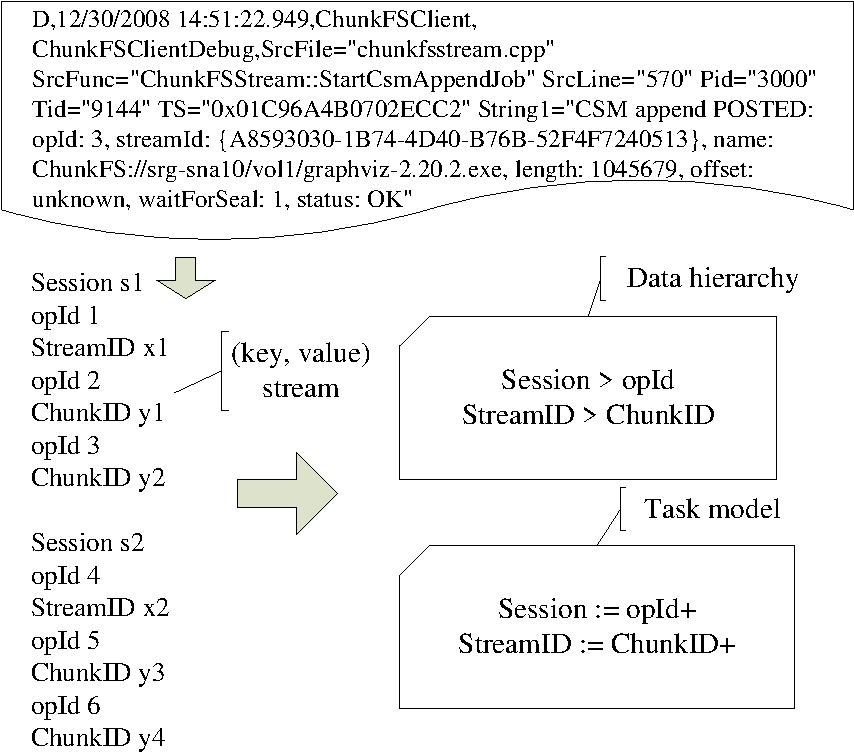
\includegraphics[height=2in]{design}
\caption{Design Overview}
\label{fig:design}
\end{figure}

Our design is summarized in Figure~\ref{fig:design}. We
first extract data from system logs as streams of (key,
value) tuples. Then we try to mine hierarchical relations
among keys. The mined relations can be directly translated
to task models. Applying the task models on logs, we
generate a set of task instances represented as an array of
log items.

\subsection{Extract key-value pairs}
\notes{value format are limited, we can find value part
easily, and track back in the text to find its key name.}

System logs contains a lot of information on system
activities. The log items mainly describes who (threads,
event handlers) are performing some operations (as function
name or in human language) on a set of data, with extra
information such as operation result (return code).

Our tool can infer the hierarchical relations among the data
on which system operates and generat task models using
inferred data hierarchy.

To do the inferrence, we have to first extract data part
from log. It will be represented as (key, value) tuples,
with key as data identifer and value as current content.

Different system have different log format. We describe how
to extract data from cosmos log in (key, value) format. The
principle described here can be adopted to analyze other
kinds of log. \notes{At the end of the section, we will
discuss this problem in general.}

\begin{verbatim}
d,12/30/2008 14:51:22.949,CosmosClient,
CosmosClientDebug,SrcFile="cosmosstream.cpp"
SrcFunc="CosmosStream::StartCsmAppendJob" 
SrcLine="570" Pid="3000" Tid="9144"
TS="0x01C96A4B0702ECC2" String1="CSM append
POSTED: opId: 3, streamId:
{A8593030-1B74-4D40-B76B-52F4F7240513}, name:
cosmos://srg-sna10/vol1/graphviz-2.20.2.exe,
length: 1045679, offset: unknown,
waitForSeal: 1, status: OK"
\end{verbatim}

The above shows a typical log item picked from cosmos.  The
cosmos log can be divided into two parts. The first half has
fixed format, which records log level, time, log category
and a short title. Followed by the location of the log in
source file, and runtime parameters. The second half is
contained in \texttt{String1} field. It is written by
developer and not well structured. It is usually interleaved
with descriptive texts and programs states in (key, value)
pairs.

It is not straightforward to extract the (key, value) pairs.
The developer can record (key, value) in several formats. In
general, it is written as \texttt{key SEP1 value SEP2}. SEP1
and SEP2 have mutiple choices. It is not easy to determine
which word is a key, otherwise we can do the job easily. A
key may look similar to an irrelevant words, such as
\texttt{POSTED:} and \texttt{opId:}.

We use a novel method to extract the (key, value) pairs. It
is based on the observation that the value part has limited
formats, such as an integer, a hexadecimal or a GUID, and it
is easy to be match by regular expression. Once the value
part is located, we can track back in the text to find its
corresponding key.

Currently, we choose to extract (key, value) pairs whose
value parts are numbers but not text. Our considerations
are: a) values as text are more descriptitive and have
little use in inferring data hierarchy in later steps. b)
SEP1 and SEP2 may be both blanks. In such cases,
text words, keys and values are messed up and they cannot be
distinguished using simple rules.

\notes{key alias: one key has multiple names, key name
collision: multiple key has the same name.  we can solve
above two problems using some key mapping scheme, but it
requires manual work and one have to familiar with log and
keys. our suggestion: regular key definition}

\subsection{Mining hierarchical relation of keys}

Some of the keys extracted from log have hierarchy
relations. For example, to complete a \texttt{Session}, it
is splitted into subtasks which are designated by different
\texttt{opId}. There are similar relations with
\texttt{StreadID} and \texttt{ExtentID}. We can use the
data hierarchy to deduce task hierarchy. Two keys have
hierarchical relations are denoted by $>$, for example,
\texttt{Session} $>$ \texttt{opId}.

After the previous step, we get a stream of (key, value)
pairs in their order of appearance in log file. Activities
from multiple threads may be logged into the same log file.
We split (key, value) streams by thread and mine different
sub-streams separately. The mined results are combined
together.

We use two heuristics to mine data hierarchy among keys.
They are the necessary conditions for two keys to have
hierarchical relation.
\begin{itemize}
\item If keyS $>$ keyP, then keyS comes before keyP.
\item If keyS $>$ keyP, then there're strict 1-to-many
mapping between keyS and keyP value set.
\end{itemize}
The intuition is, if keyS $>$ keyP, one will see keyS first,
and a series of keyP with different values, and then keyS,
with another value, and then a series of keyP. 

The mining algorithm takes (key, value) stream as input and
outputs (keyS, keyP, R) tuples, indicating keyS $>$ keyP
with rank R.

\begin{verbatim}
A a1
B b1
B b2
A a2
B b3
\end{verbatim}
\notes{this will replaced by example below}

There above (key, value) streams servers as an simple demo
of mining algorithm. After mining, we will get (A, B, 3).
Because A appears before B, A is a possible parent of B. The
rank 3 is calulated as the cardinality of (valueA, valueB)
set: \{(a1, b1), (a1, b2), (a2, b3)\}

The rank algorithm works as follows. It scans through the
(key, value) stream and maintains an array of keys. Once a
key is spotted for the first time, it is appended to the key
array. A key is a possible parent for all the keys after it
in the array (heuristic 1). In the scan process, the algorithm also
accumulate an array of (valueS, valueP) for each (keyS, keyP)
pairs. A new (keyP, valueP) will generate multiple (valueS,
valueP) for each keyS before keyP in the key array.

Now for each (keyS, keyP) pair, we have a corresponding
(valueS, valueP) array. To apply heuristic 2, we have to
justify whether valueS and valueP have strict 1-many
mappings. If yes, we use size of (valueS, valueP) array
as the rank of (keyS, keyP), if not, we just ignore the
(keyS, keyP) pair.

\notes{pseudo code of mining algorithm}

We give a more complete example here.
\begin{verbatim}
Session s1
opId 1
StreamID x1
opId 2
ExtentID y1
opId 3
ExtentID y2

Session s2
opId 4
StreamID x2
opId 5
ExtentID y3
opId 6
ExtentID y4
\end{verbatim}
The above example emulate the (key, value) stream we see in
cosmos client log. When the client receives a command, it
starts a new session, opens the specified stream in next
operation step, and process extents of the stream in the
following operation steps.

We sucessfully mined out StreamID $>$ ExtentID with rank 4
and Session $>$ opId with rank 6. Session has no relation
with StreamID, because multiple Session may operate on the
same StreamID. The similar argument apply for (Session,
ExtentID), (opId, StreamID) and (opId, ExtentID).

For (key, value) streams generated form real world log, the
mined result may contain a lot false positives.

\notes{Have to find some way to automatically filter out
false positives. For example, if (err, 0x0) is inserted
after each Session, we will see Session $not >$ err, but
err $>$ opId and Session $>$ opId, using transitive rule?}

\notes{cannot reduce all false positives. patch 1: user
specify a subset of all keys. patch 2: user manually delete
false pairs}

\subsection{Construct hierarchical task models}

\notes{task model can be expanded to many task instances. The
boundary of a task instance defined by value flip point.}

After the previous step, we mined out a set of data
hierarchy relations. The relations can be translated
directly to hierarchies of tasks which process the data. 
If we have keyS $>$ keyP, and use Task(keyS) to denote task
that process keyS, then we have Task(keyS) $:=$
Task(keyP)$+$, in short keyS $:=$ keyP+

We apply the mined data hierarchy on the log to construct
task models. We first split log items into groups by highest
level key. The group begins at the new value of a key and
last until another value is met. We apply the process
recursively within each group to construct hierarchical task
models.

%join the pairs together

The choice of which data hierarchy to apply is left to user.
The choice depends on user's concentration. The user are not
limited to mined result. Other hierarchy relations can be
specified. For example, one can combine Session, opId,
StreamID, ExtentID together, and write the relation as
Session $:=$ opId$+$, opId $:=$ StreamID$|$ExtentID.

\notes{the result task boundary is an approximation, has a
shift with `real' boundary.}

\subsection{Put things together}

From the demo to task model and then task instances



%% vim:tw=60

\section{Discussion}
\label{sec:discussion}
Discussion. \notes{topic need decided}

dependency line cannot be draw from log

we can overlay the task model on scapel to a) see how high
level tasks are mapped to low level synchonization
operations, b) see dependency among tasks

Or we can put a short discussion paragraph at the end of
each subsection of Design section.


\section{Implementation}
\label{sec:impl}

We implement a prototype of SMON system on Planet-Lab.  The
source is written in Python, and the final installation
package size of a BON peer is about 122KB, with 1000+ lines
of code.

\begin{table*}
\small
\centering
\begin{tabular}{|l|l|}

\hline
\textbf{RPC} & \textbf{Description} \\

\hline
\texttt{ping(ver)} & Call with local SMON peer's version and
return remote peer's version.\\

\hline
\texttt{retrieve\_peer(ver)} & Retrieve installation package
of SMON peer with specified version.\\

\hline
\texttt{exchange\_livetag(tag, ver)} & Call with local
$<$livetag, version$>$, and return remote peer's $<$livetag,
version$>$.\\

\hline
\texttt{exchange\_member(ver)} & Call with local membership
list version and return remote peer's membership list.\\

\hline
\texttt{retreive\_member(ver)} & Retrive membership list of
specified version.\\

\hline
\texttt{exchange\_app(app\_name)} & Call with an application
name, return true if remote peer has installed the
application.\\

\hline
\texttt{retrieve\_app(app\_name)} & Retrieve installation package
of an application with specified name.\\

\hline
\texttt{resolve\_challenge(challenge)} & Return the response
to an authentication challenge.\\

\hline
\texttt{set\_app\_status(app\_name, status)} & Set application status (online,
offline, ignore).\\

\hline
\texttt{get\_app\_status(app\_name)} & Get application status. \\

\hline

\end{tabular}
\caption{RPC interfaces of SMON peer and authentication
agent}
\label{fig:rpc}
\end{table*}

The epidemic activities of a SMON peer is implemented in
several
threads, including one for monitoring and maintaining other
peers, one for updating membership list, one for update
\texttt{livetag}. For each application, a separate thread
will be started for maintaining the application.

The communication with peers and agents are implemented as
RPCs, and they are summarized in table~\ref{fig:rpc}.


SMON peer copies installation packages or executes commands
by spawning a ssh/scp process. A modified \texttt{ssh-agent}
is started which forwards the authentication challenge from
ssh/scp to the remote authenticate agent. The agent only
implements one RPC interface \texttt{resolve\_challenge}
described in table~\ref{fig:rpc}.

The parameters used at SMON runtime is stored in a
configuration file. It stores the time intervals among
consecutive epidemic activities, the version numbers for
SMON peer and membership list, the $<$livetag, version$>$
tuple, the address of authentication agent. Each application
can specify an address to which the application's states
changes should be reported. The configuration file is
implemented as a SQLite database file to avoid data loss at
machine crash. It is updated by
installation package of SMON and applications.  The
membership list is stored separately in compressed format.

%SMON makes a predefined and consistent directory layout of
%peer installation and it is critical for peers to perform
%their functions correctly. A SMON peer is installed to
%\texttt{SMON} directory of user's home directory, and this
%setting can be changed. Under \texttt{bin} directory, a
%\texttt{run.py} and \texttt{smon.cfg} is placed. To start
%SMON peer, \texttt{run.py} is executed and it read
%configuration in \texttt{smon.cfg} and start the version
%specified in \texttt{smon.cfg}. A new version SMON peer
%should change \texttt{smon.cfg} appropriately. Different
%version of SMON peer is placed according to version number
%under different directories. \texttt{app} directory contains
%different application entries, as different directories. A
%configuration file for each application is placed under it
%directory. Installation package of SMON peer and
%applications are stored under \texttt{packages} directory,
%placed according to its name and version.

%ping interval and timeout value

% vim:foldmethod=marker:textwidth=60

\section{Analysis}
\label{sec:analysis}

We analyze performance of SMON in this section.

SMON uses epidemic algorithm to maintain itself. Peers will
initiate periodic communication to other random peers. We
will show that these maintenance tasks have good
performance and scalability. In the analysis, we assume that
SMON works in synchronized way, that is each peer performs
its maintenance tasks in synchronized rounds and the tasks
finish almost instantaneously. Although the real SMON system
works asynchronously, the analysis can still give insights
on performance of SMON design. We will also evaluate SMON in
real conditions (see section~\ref{sec:eval}) and validate
our analysis.

% performance and scalability

The epidemic algorithm has three variants, called push, pull
and push-pull, and they are used by different maintenance
tasks of SMON.
%as summarized in table~\ref{tbl:tasks}.
Although they differ in details, the basic result of
epidemic theory shows that each one of the three methods can
eventually infect the entire population.  The studies also
show that starting from a single peer, this is achieved in
expected time (the rounds number) proportional to the log of
the population size ($\log N$).

%\begin{table}
%\centering
%\begin{tabular}{|l|l|}
%
%\hline
%Self-deployment & push \\
%
%\hline
%Self-upgrade & push-pull \\
%
%\hline
%Self-recovery & push \\
%
%\hline
%Enable SMON & push \\
%
%\hline
%Disable SMON & pull \\
%
%\hline
%Application deployment & push-pull \\
%
%\hline
%\end{tabular}
%\caption{Different variants of epidemic algorithm used by
%maintenance task of SMON.}
%\label{tbl:tasks}
%\end{table}

Take self-deployment process as an example. Starting from a
single SMON peer, all the target machines will be deployed
with a SMON peer.  According to existing
studies~\cite{Eugster2004}, the self-deployment process can
be modeled as a branching process with population $n$. After
$r$ rounds, the expected fraction of deployed machines is
\begin{equation*}
Y_r \approx \frac{1}{1+ne^{-r}}
\end{equation*}
The relation of $Y_r$ and $r$ is demonstrated in
figure~\ref{fig:yr}.

\begin{figure}
\centering
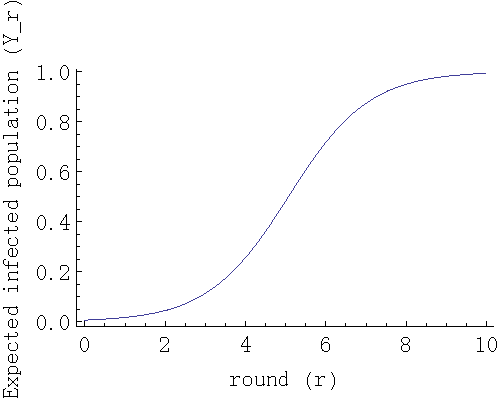
\includegraphics[scale=0.618]{Y_r}
\caption{Relation of expected infected population $Y_r$ with
round number $r$.}
\label{fig:yr}
\end{figure}

From the equation above, the ratio of deployed machines to
un-deployed ones increases exponentially, on average, by a
factor of $e$ in each round.  This indicates that the
self-deployment has good performance.
%
%To deploy a fix fraction of machines, the expected round
%number $r$ is:
%
%\begin{equation*} r \approx \ln(n) - \ln(\frac{1}{Y_r} - 1)
%\end{equation*}
%
%$r$ is in the logarithm of total population $n$, which
%implies good scalability of self-deployment process.

% overhead number

Another performance metric in concern is the overhead in
the self-deployment process. Since we use epidemic
algorithm, there may be duplicated deployed SMON peers in a
machine. Although there will be only one instance running,
the duplicated deployment will waste network resource and
disk storage at some extent.

We next show that the overhead is small on average (constant
actually). Assuming that there are $n$ machines in total,
and $m$ machines have been deployed already. For any one of
$n-m$ un-deployed machines, it may be selected by $k, (k <=
m)$ peers as the deployment target in the next round.  The
distribution of $k$ is can be expressed as binomial
distribition with parameter $(m, \frac{1}{n})$
\begin{equation*}
P(X=k) = C_m^k (\frac{1}{n})^k (1 - \frac{1}{n})^{m - k}
\end{equation*}
We define the simultaneous deployment number $k, (k > 0)$ as
the deployment overhead. It is the conditional probability
when $k > 0$
\begin{equation*}
\begin{aligned}
P(X' = k) &= P(X=k | X > 0) \\
%&= P(X = k) / (1 - P(X = 0)) \\
&= P(X = k) / (1 - (1 - \frac{1}{n})^{m}) \qquad (k > 0)
\end{aligned}
\end{equation*}
The expectation of $k$, the overhead number, is
\begin{equation*}
\begin{aligned}
E(X') &= \sum_{k=1}^m k \cdot P(X=k|X>0)  \\
      &= \frac{1}{(1 - (1 - \frac{1}{n})^{m})} E(X)
\end{aligned}
\end{equation*}
Further, note that when $n$ is large, and $m$ is approaching
$n$, we have
\begin{equation*}
\lim_{n \to \infty, m \to n} (1 - \frac{1}{n})^{m} = 1 / e
\end{equation*}
Thus,
\begin{equation*}
\begin{aligned}
E(X') &\approx 1.582 \cdot E(X) \\
      &= 1.582 \times \frac{m}{n}
\end{aligned}
\end{equation*}
And finally, we have
\begin{equation*}
\lim_{n \to \infty, m \to n} E(X') = 1.582
\end{equation*}
This shows that the average overhead number will approach a
constant value when SMON is deployed at large scale.

At last, we show that the average number of ping messages
received by any peer is also constant.  When SMON is running
on $n$ peers, the number of ping messages $p$ received by a
SMON peer is in the binomial distribution of parameter $(n,
1/n)$. Thus we have
\begin{equation*}
E(p) = n \cdot 1/n = 1
\end{equation*}

% ping overhead

% At last, we show that the communication cost caused by
% maintenance tasks is small. At each round, a SMON peer will
% selecte a random peer and send it two messages: a ping
% piggybacked with version number

% recover speed?


% vim:foldmethod=marker:textwidth=60

\section{Evaluation}
\label{sec:eval}

We conducted experiments on Planet-Lab platform to evaluate
SMON system, and compare the results with analysis in
section~\ref{sec:analysis}. Planet-Lab is a global research network
consisting of 900+ nodes at 400+ sites around the
world.

%let SMON start self-deployment. We study the performance of
%the self-deployment process, and measure the overhead
%introduced in solving race conditions. To show SMON has
%good scalability, we deploy SMON on another set of 24
%nodes, and compare the performance with the previous
%deployment. We then close SMON by ... and study the
%performance ...
%
%Our experimental results show that SMON is efficient at
%deploying itself and achieves good scalability, the
%overhead caused by race condition is small and the active
%state transition is fast.

We evaluate the performance of self-management design. As
the maintenance tasks performed by SMON peer to deploy,
recover and upgrade the system use the same epidemic
algorithm, we only present the results on self-deployment
and enabling a disabled SMON system. 

\begin{figure}[t]
\centering
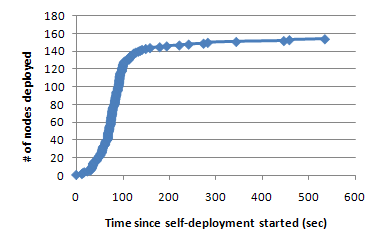
\includegraphics[scale=0.618]{self-deploy.png}
\caption{Progress of self-deployment process on 159
nodes.}
\label{fig:self-deploy}
\end{figure}

First, we evaluate the performance of self-deployment of
SMON.  We choose 159 nodes in Planet-Lab platform and start
a SMON peer. SMON then start deploying itself on all 159
nodes.

In our configuration, A SMON peer detects a random nodes and
sleep for 5 seconds. We finally collected data from 154
nodes out of 159 nodes. There are 5 nodes unreachable at
data-collecting stage and their data are omitted in the
result. This kind of failure is common for large scale
distributed systems.  Figure~\ref{fig:self-deploy} shows the
progress of self-deployment. We can see that 90\% (143) of
nodes are deployed successfully with a SMON peer within 149
seconds. The median deployment time is 93 seconds while the
largest one is 533 seconds. As a comparison,
figure~\ref{fig:self-deploy} has similar trends with
analysis result (figure~\ref{fig:yr}). But
figure~\ref{fig:self-deploy} exhibits an obvious long tail.
The long tail in figure~\ref{fig:self-deploy} are caused by
two reasons: either the network to the machine is slow or
the the machine itself is overloaded and doesn't respond
quickly.

We then evaluate the performance of enable/disable
self-management functionality of SMON system. We first
disable self-management of SMON system deployed on 159
Planet-Lab and then enable it again. The progress of state
transition from disabled to enabled is shown in
Figure~\ref{fig:state-transition}. For 90\%
percentile of peers, the states changes after 143
seconds and the median state transition time is 37 seconds.

%\begin{table}
%\centering
%\begin{tabular}{|l|c|}
%\hline
%median & 37 \\
%\hline
%90\% percentile & 143 \\
%\hline
%\end{tabular}
%\caption{Statistics for state transition experiment in seconds}
%\label{tbl:state-transition}
%\end{table}

\begin{figure}[t]
\centering
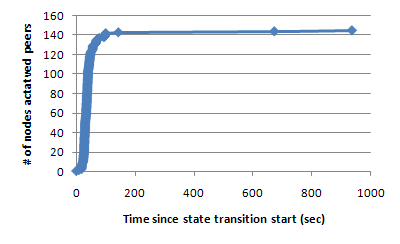
\includegraphics[scale=0.618]{state-trans.png}
\caption{Progress of state transition of self-management from disabled to
enabled.}
\label{fig:state-transition}
\end{figure}

To evaluate the scalability of self-deployment process, we deploy
a new instance of SMON system at a different scale (24 nodes) and
compare the performance of self-deployment process.
Table~\ref{tbl:scalability} summarizes the statistics results.
We can see from the table that the scalability is good.
While scale difference between two systems is about 6.6
(159/24) times, the
90-percentile deployment time is only 1.75 (149/85) times of
difference, while the median value is 1.41 (82/58) times of
difference. The above two ratios is close to the ratio of
logarithm of system scales ($\log 159 / \log 24 = 1:59$).

\begin{table}
\centering
\begin{tabular}{|l|c|c|}
\hline
  & 24 nodes & 159 nodes\\
\hline
median & 58 sec & 82 sec \\
\hline
90\% percentile & 85 sec & 149 sec\\
\hline
Final & 103 sec & 533 sec\\
\hline
\end{tabular}
\caption{Comparison of self-deployment process at different
scales in seconds.}
\label{tbl:scalability}
\end{table}

During the self-deployment process, there are cases that
multiple SMON peers try to deploy an instance on the same
node and this can cause extra overhead. The overhead wastes
network bandwidth and the storage at the deployed node. We
evaluate the overhead by count the simultaneous deployment
happened at each node. The result is shown in
Figure~\ref{fig:overhead}. We can see that for 43.71\% of
nodes there is exactly one deployment on each of them.
Obviously, most of nodes have a deployment overhead within
10. These nodes account for 92.04\% of all nodes and the
average overhead of these nodes is 2.31. The average
overhead for all nodes is 4.30 which is an acceptable
number. The number 4.30 is larger than the analysis result
(1.582) in section~\ref{sec:analysis}. The reason is that,
in the analysis we assume that SMON works synchronously but
the real system works asynchronously and the deployment
takes time. During the time a peer chooses a machine to
deploy a new peer, other peers will choose the same machine
and don't notice the simultaneous deployment. This will
cause greater overhead number than analysis.

\begin{figure}
\centering
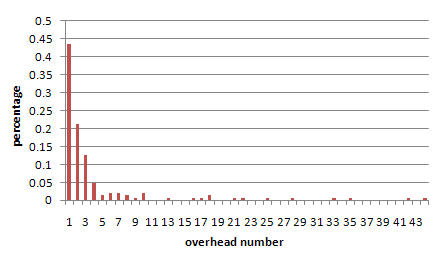
\includegraphics[scale=0.5]{overhead.png}
\caption{Overhead (copy number of simultaneous deployment)
introduced by race condition during
self-deployment process}
\label{fig:overhead}
\end{figure}


% vim:foldmethod=marker:textwidth=60

% vim:tw=60

\section{Related Works}
\label{sec:related}
Related Works \cite{Lamport1978}



% vim:tw=60

\section{Conclusion}
\label{sec:conclusion}
Conclusion



\bibliographystyle{IEEEtran}
\bibliography{ref}

\end{document}

% vim:foldmethod=marker:textwidth=60
